\lettrine{T}{his appendix chapter} includes some additional information about the models I have run. I include this to discuss some of the notable features and challenges to the models, and how I account for this.

\section{Variation: \textit{Regime}}
I include two plots showing the variation in the freedom of expression (dependent) variable and the FBIC (independent) variable for each regime type. I use a violin plot to see how the observations cluster along the range of the variable for each regime type. I also include a table with different information for each of the four regime types. I find that there is enough variation for the variables to be useful, although I would have liked more variation in the linkage variable.

\begin{table}[H]
\centering
\caption{Information on freedom of expression and linkages scores for each regime type}
\label{tab:variation}
\resizebox{\textwidth}{!}{
\begin{tabular}[t]{lrrrrrrrr}
\toprule
\multicolumn{1}{c}{ } & \multicolumn{2}{c}{Closed Autocracy} & \multicolumn{2}{c}{Electoral Autocracy} & \multicolumn{2}{c}{Electoral Democracy} & \multicolumn{2}{c}{Liberal Democracy} \\
\cmidrule(l{3pt}r{3pt}){2-3} \cmidrule(l{3pt}r{3pt}){4-5} \cmidrule(l{3pt}r{3pt}){6-7} \cmidrule(l{3pt}r{3pt}){8-9}
  & Freedom & Fbic & Freedom & Fbic & Freedom & Fbic & Freedom & Fbic\\
\midrule
Mean & 0.281 & 0.515 & 0.820 & 0.937 & 0.091 & 0.101 & 0.059 & 0.051\\
SD & 0.253 & 0.221 & 0.077 & 0.049 & 0.091 & 0.093 & 0.059 & 0.039\\
Min & 0.012 & 0.026 & 0.526 & 0.653 & 0.000 & 0.000 & 0.000 & 0.001\\
Max & 0.904 & 0.919 & 0.958 & 0.989 & 0.432 & 0.479 & 0.346 & 0.286\\
\bottomrule
\end{tabular}
}
\end{table}

\subsection{Freedom of expression}
In Figure \ref{fig:variation_freedom} both closed and electoral autocracies are spread out along almost the entire length of the freedom of expression variable. The shape is long and thin, meaning that they do not seem to cluster at certain points. The shapes for electoral and liberal democracies are wider and more concentrated, giving them less variation. However, all four regime types exhibit a good deal of variation in freedom of expression.

\begin{figure}[H]
    \centering
    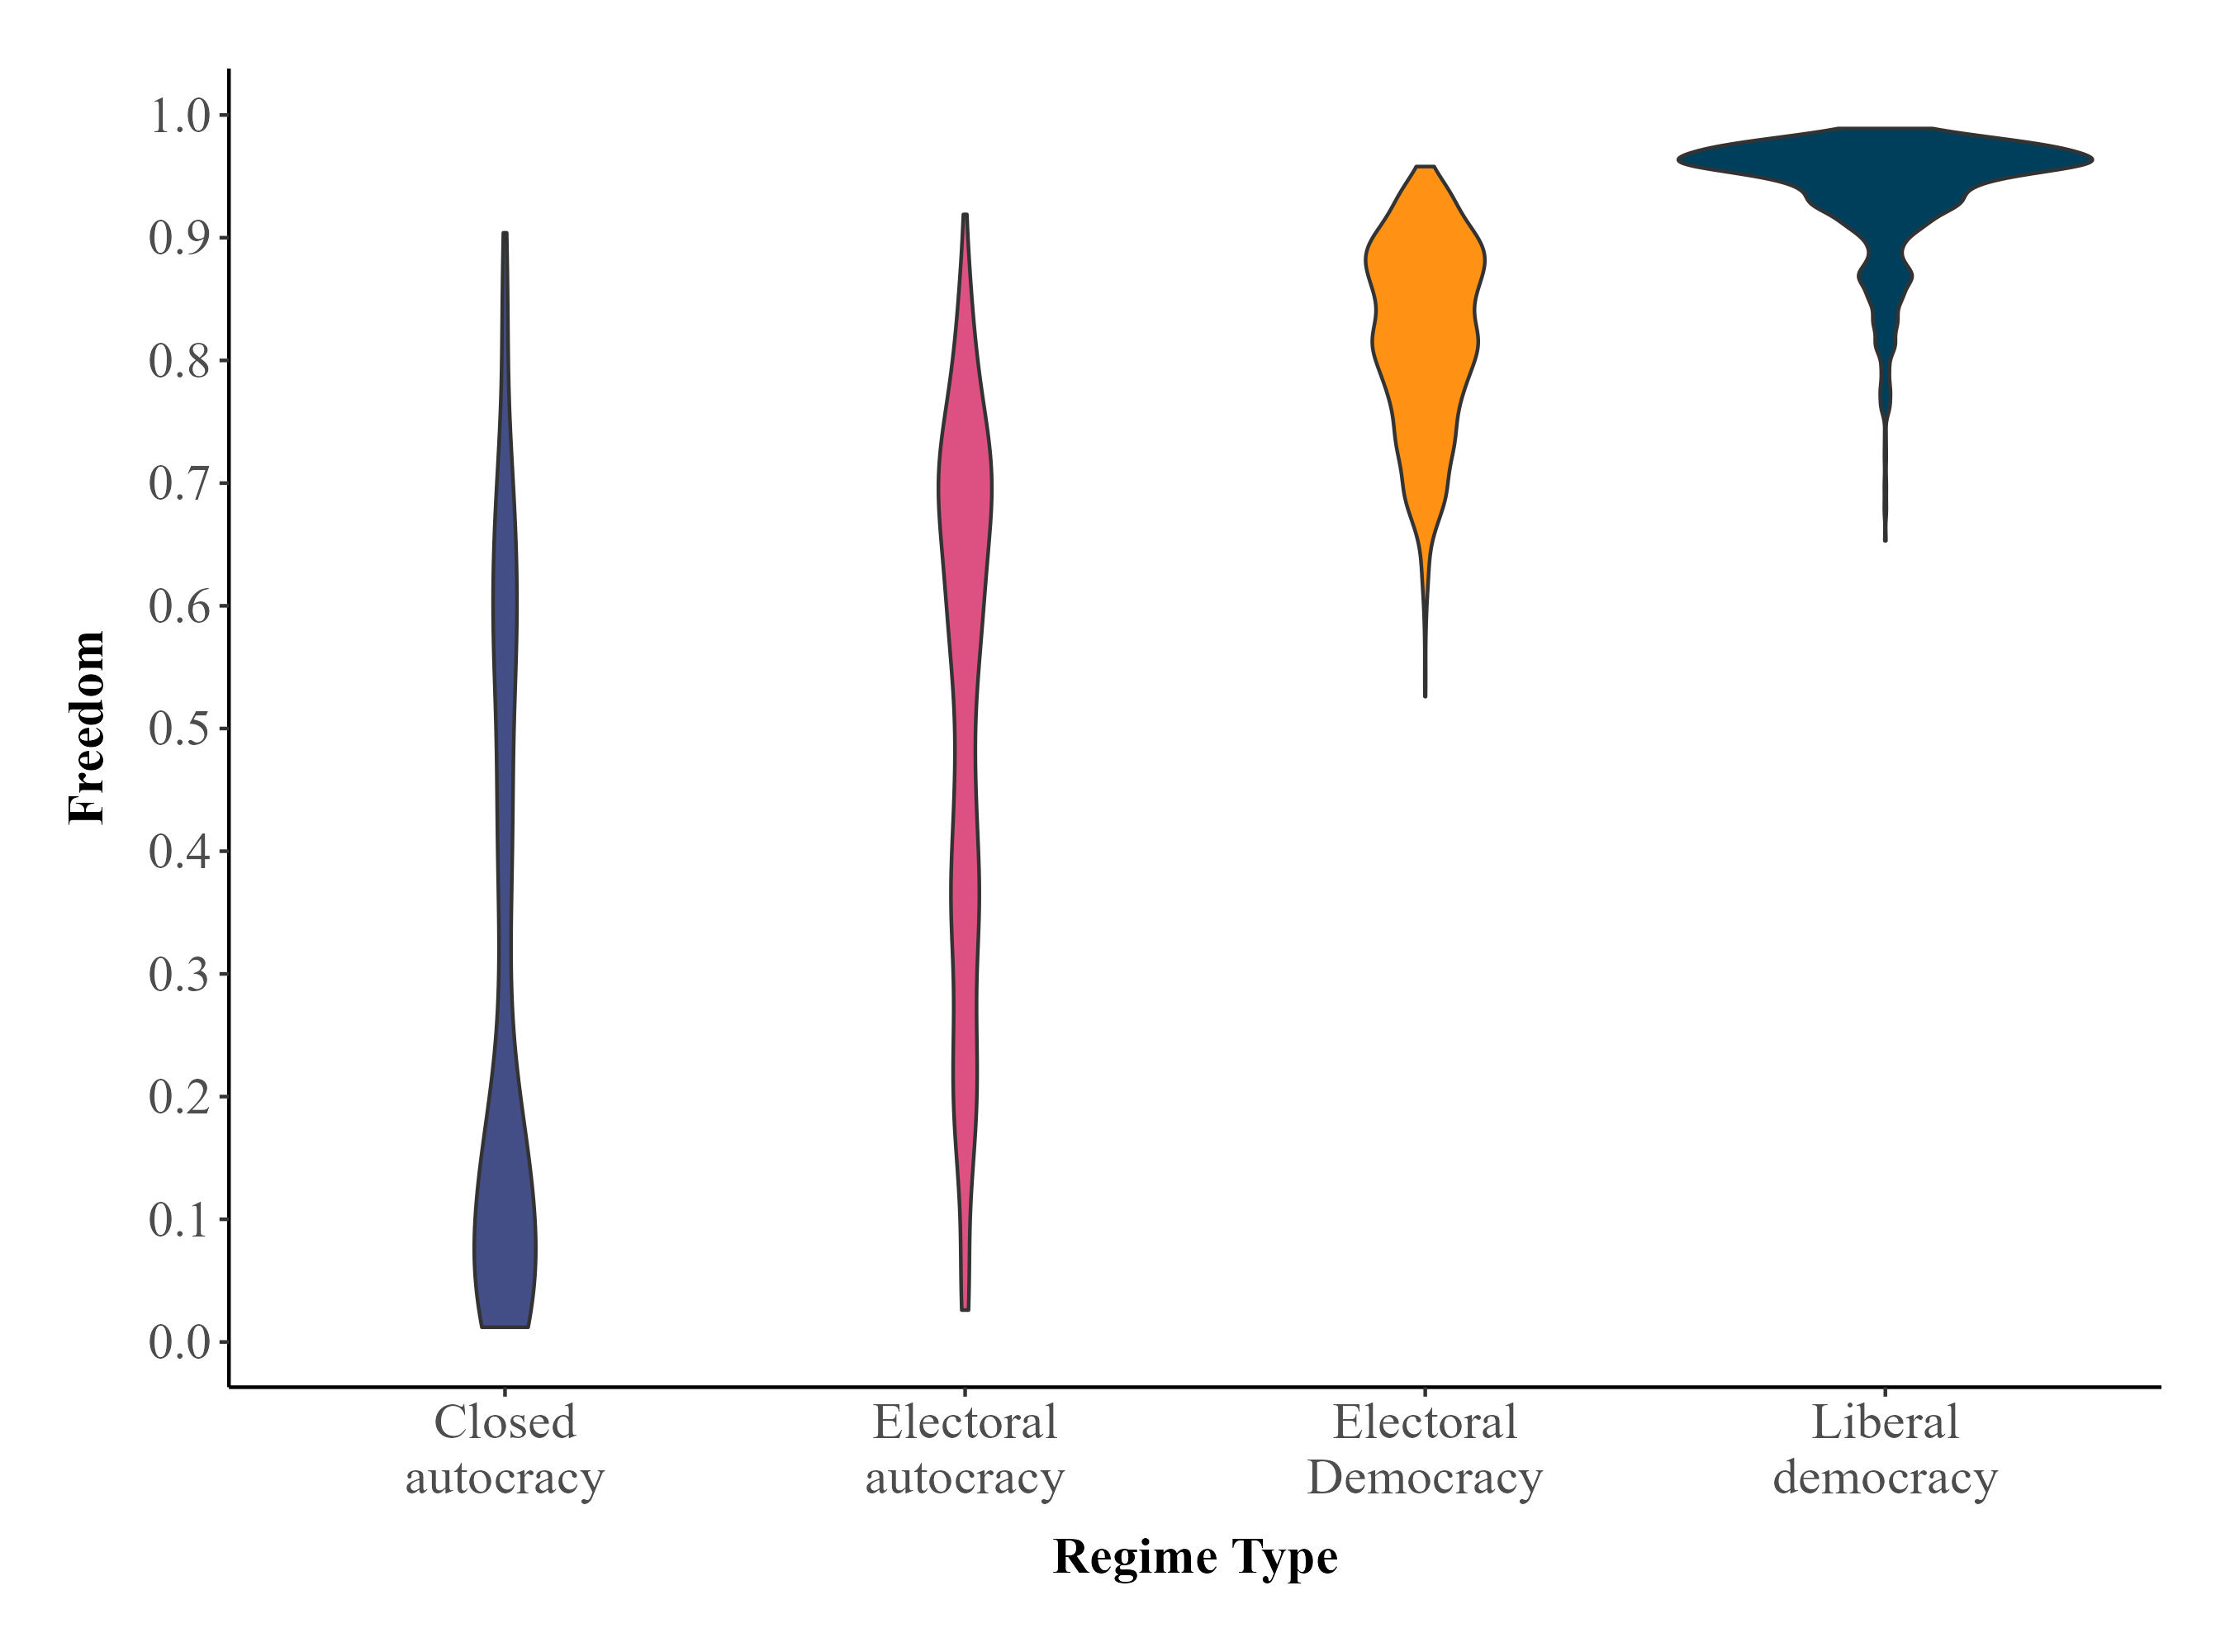
\includegraphics[width=\linewidth]{graphics/variation_freedom.jpeg}
    \caption{Variation in the freedom of expression score for each regime type}
    \label{fig:variation_freedom}
\end{figure}

\subsection{Linkages}
In Figure \ref{fig:variation_fbic} there is clearly less variation, with values tending to cluster at around zero. There is difference among the categories, with electoral autocracies having the most variation, and electoral democracies having the least. Generally, the autocracies have more variation than the democracies, as was the case for Figure \ref{fig:variation_freedom}. There is, however, enough variation to make this variable interesting to study for all regime types. 

\begin{figure}[H]
    \centering
    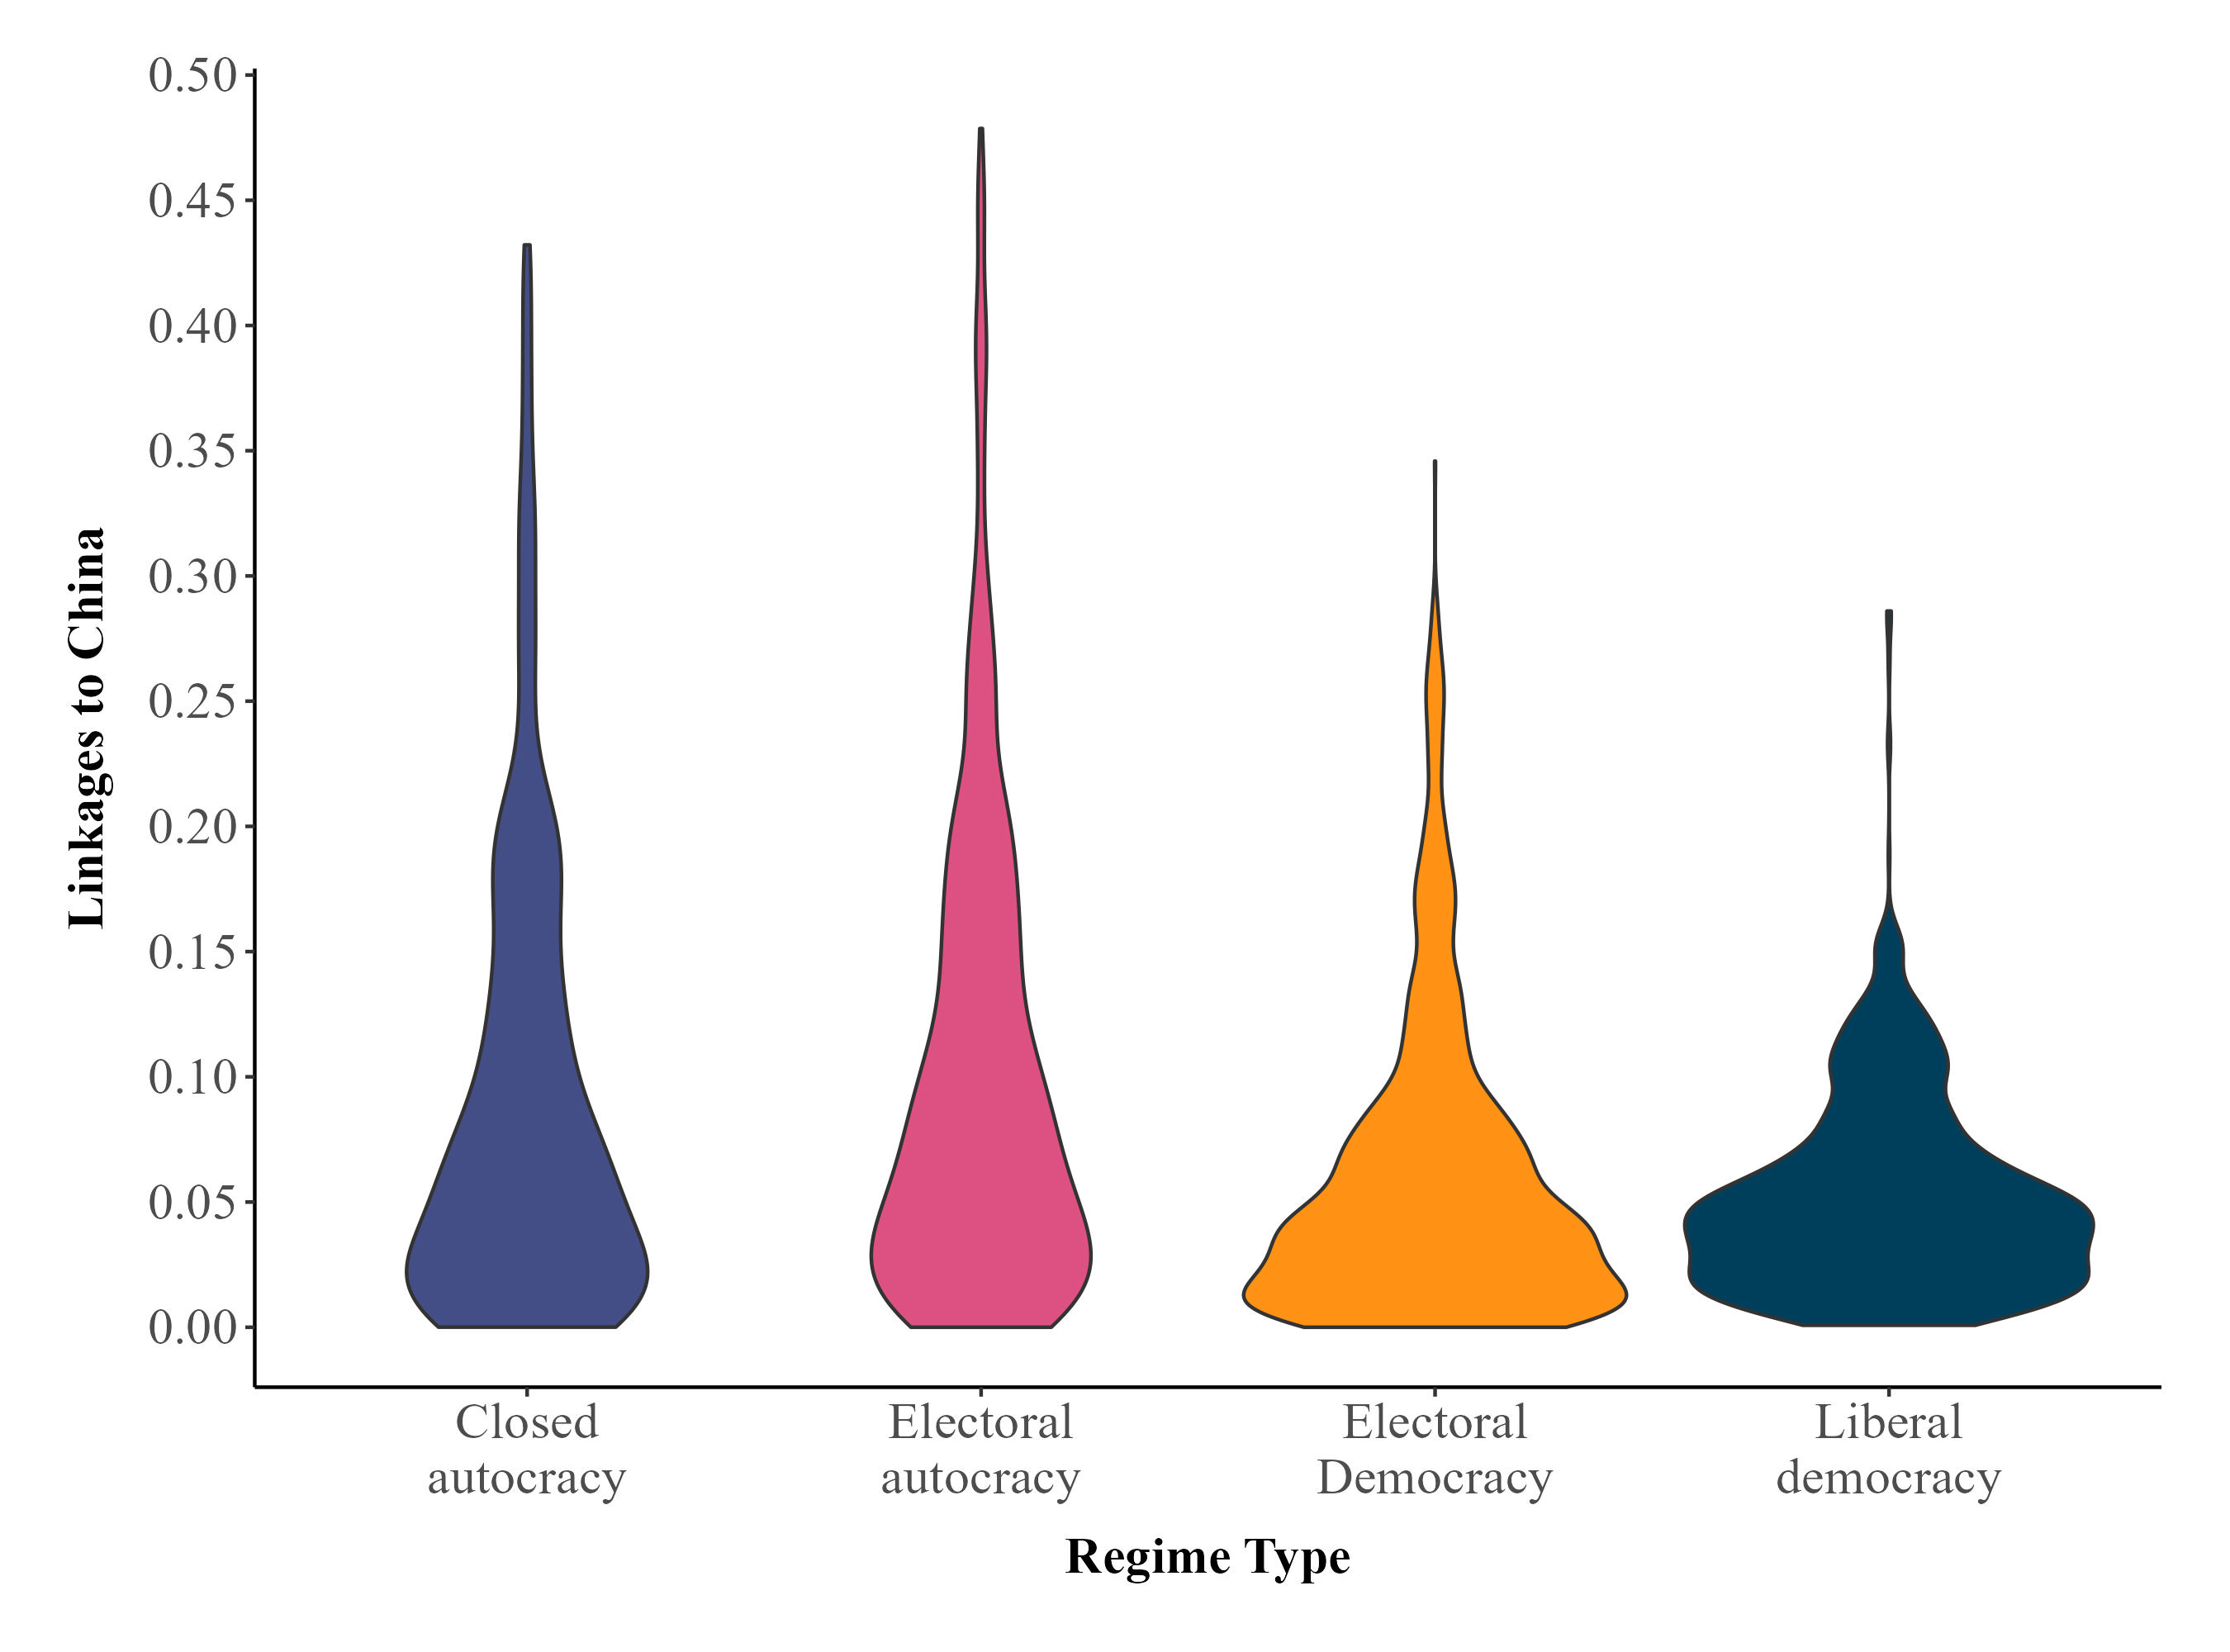
\includegraphics[width=\linewidth]{graphics/variation_fbic.jpeg}
    \caption{Variation in the linkage score for each regime type}
    \label{fig:variation_fbic}
\end{figure}

\newpage

\section{Residuals}
I here display the residual plot of Model 2.5 in Table \ref{tab:h2}. The residuals are quite similarly distributed in all the main plots. There is a very distinct shape to the plot, but there are two important ting to note: one, the model is unbiased, and two, this problem of heteroscedasticity can be solved by using clustered standard errors.

\begin{figure}[H]
    \centering
    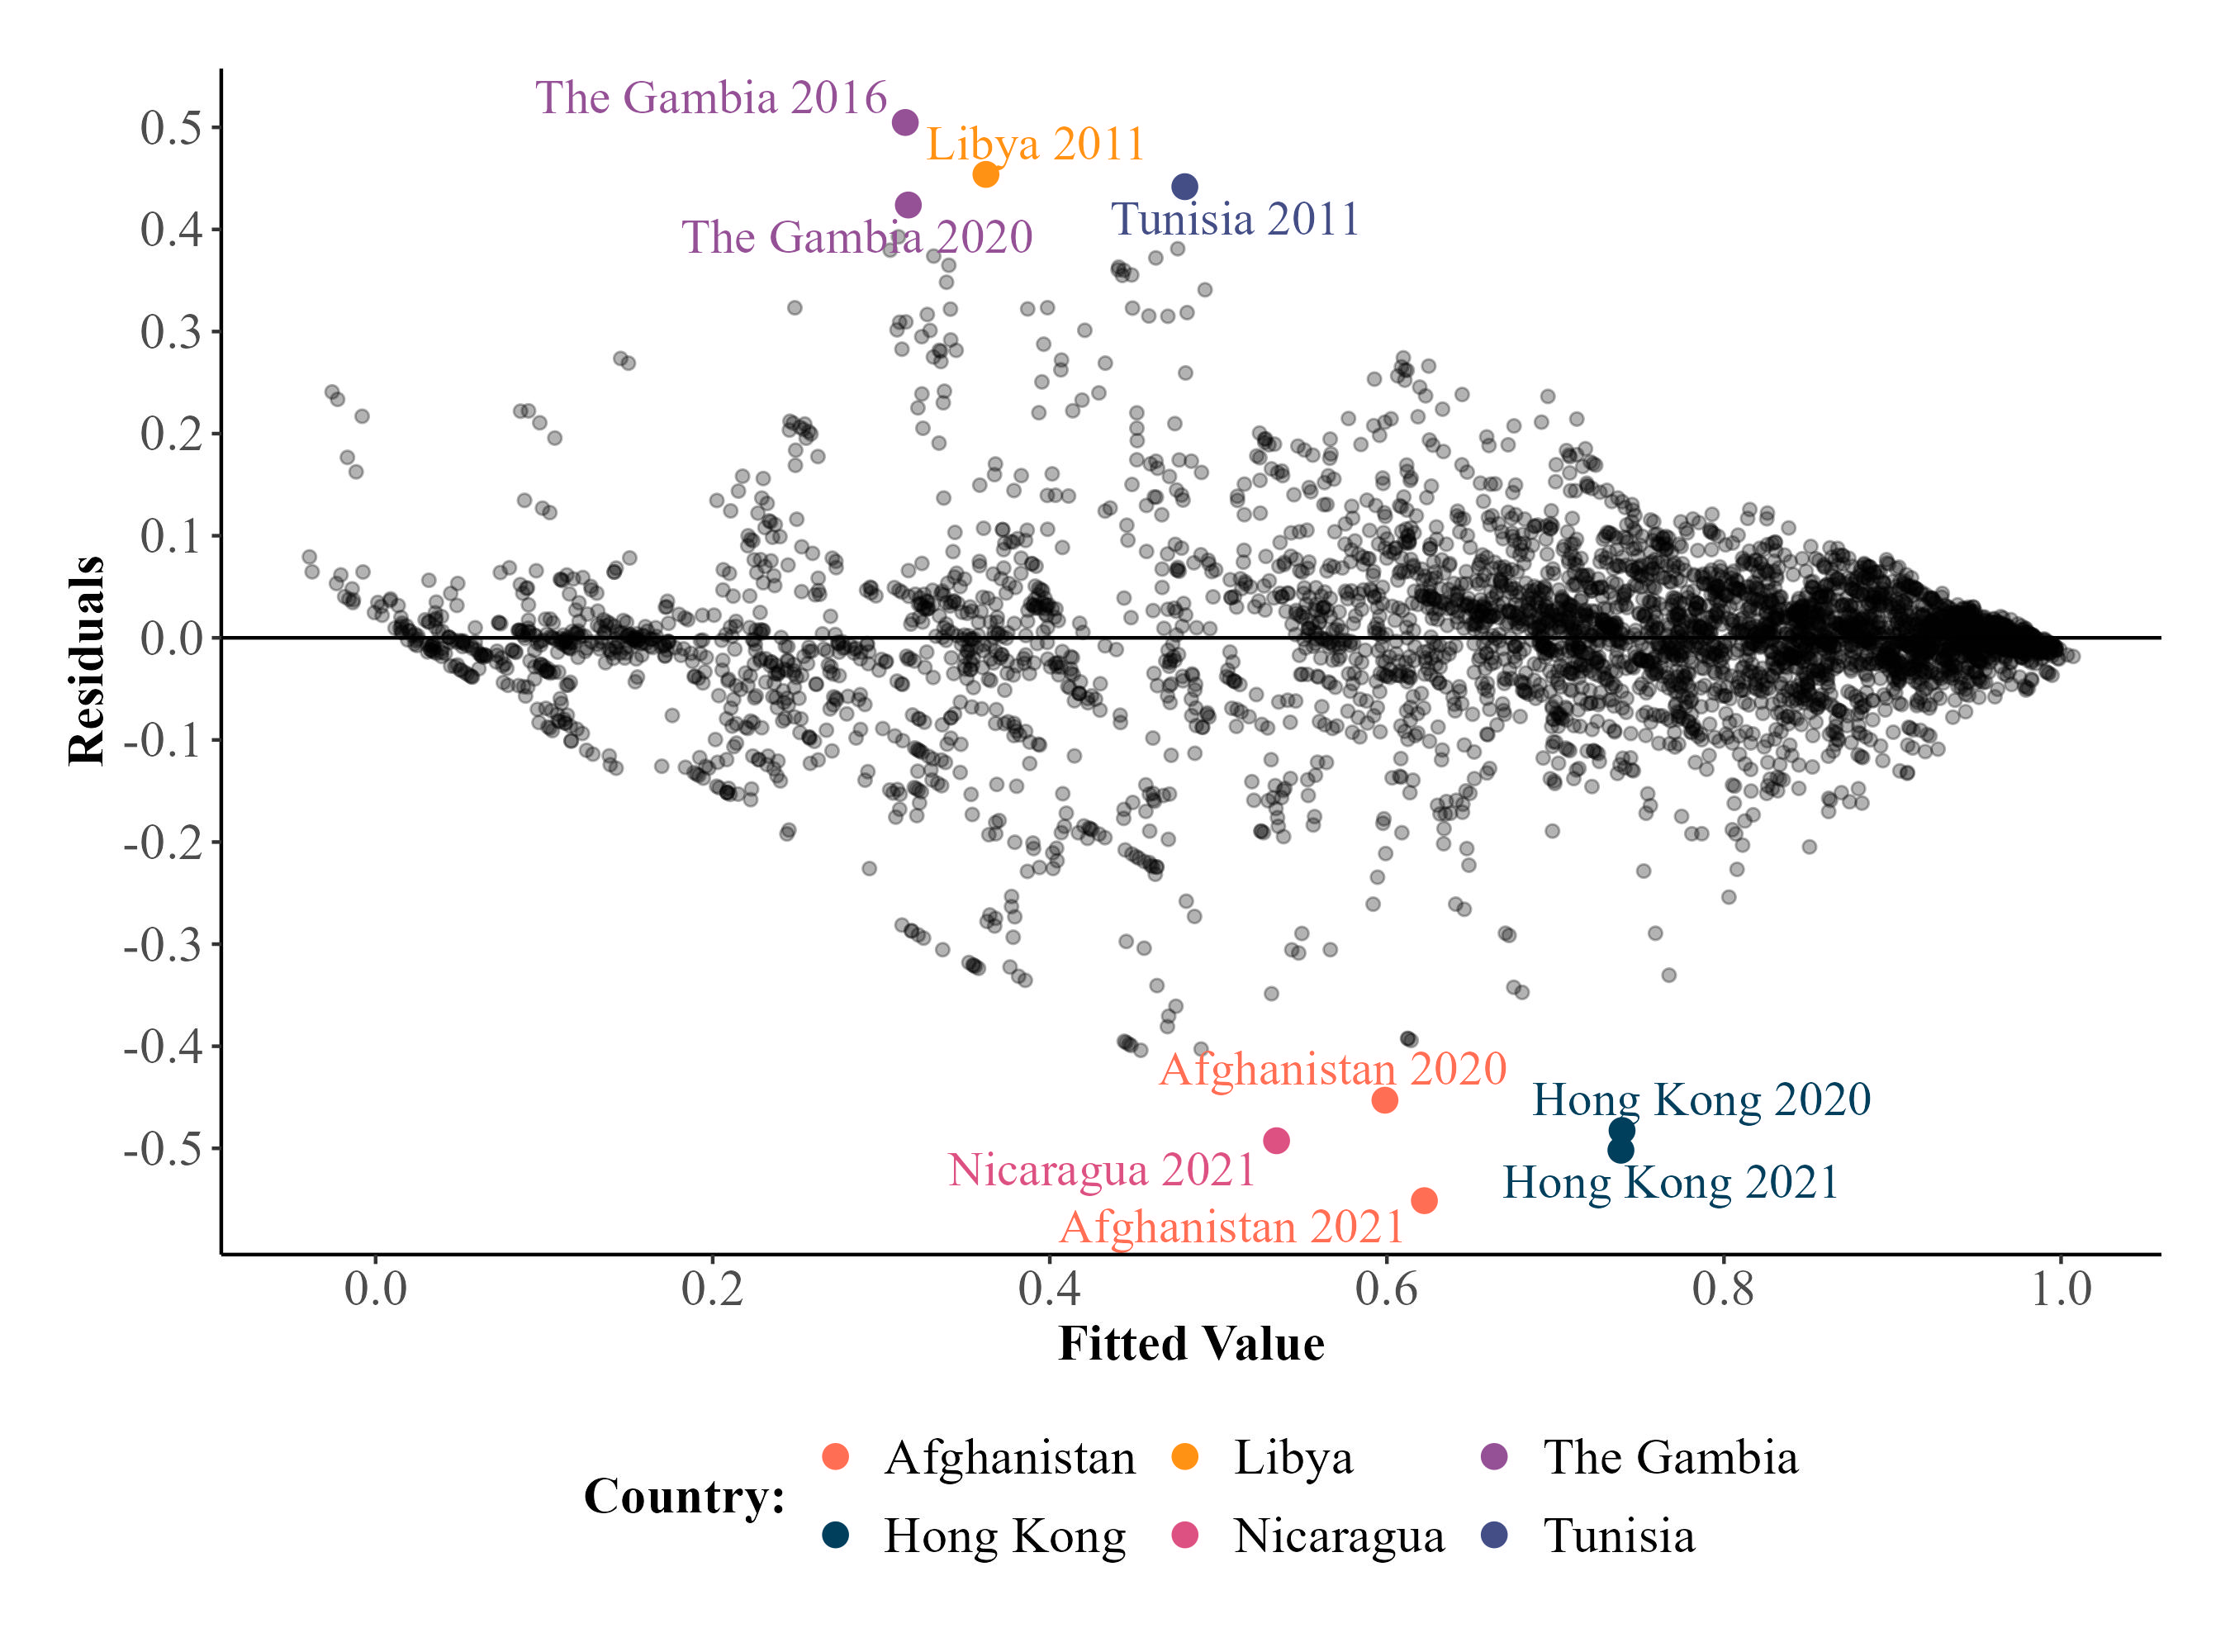
\includegraphics[width=\linewidth]{graphics/residuals.jpeg}
    \caption{Residual plot for Model 2.5}
    \label{fig:residuals}
\end{figure}